\documentclass{llncs}
\usepackage[utf8]{inputenc}
\usepackage[noend]{algorithmic}
\usepackage{algorithm}
\usepackage{epsfig}
\usepackage{multicol}
\usepackage{multirow}
\usepackage{wrapfig}
\usepackage{subfigure}
\usepackage{url}
\newcommand{\verbatimproperties}{\renewcommand{\baselinestretch}{0.85} \small}
%\newcommand{\tableproperties}{\centering \big}
\newcommand{\LINECOMMENT}[1]{$\triangleright$ #1}

%\setlength{\belowcaptionskip}{-26pt}

%%%%%%%%%%%%%%%%%%%%%%%%%%%%%%%%%%%%%%%%%%%%%%%%%%%%%%%%%%%%%%%%%%%%%%

\begin{document}

\title{On Extending a Full-Sharing Design with Batched Scheduling}

\author{Miguel Areias \and Ricardo Rocha}

\institute{CRACS \& INESC TEC and Faculty of Sciences, University of Porto\\
           Rua do Campo Alegre, 1021, 4169-007 Porto, Portugal\\
           \email{\{miguel-areias,ricroc\}@dcc.fc.up.pt}}

\maketitle

%%%%%%%%%%%%%%%%%%%%%%%%%%%%%%%%%%%%%%%%%%%%%%%%%%%%%%%%%%%%%%%%%%%%%%

\begin{abstract}

  \textbf{Keywords:} Multithreading, Tabling, Concurrency, Batched
  Scheduling
\end{abstract}

%%%%%%%%%%%%%%%%%%%%%%%%%%%%%%%%%%%%%%%%%%%%%%%%%%%%%%%%%%%%%%%%%%%%%%
\section{Introduction}

Tabling~\cite{Chen-96} is an implementation technique that overcomes
some limitations of traditional Prolog systems in dealing with
redundant sub-computations and recursion. Tabling consists of storing
intermediate answers for subgoals so that they can be reused when a
repeated subgoal appears during the resolution process. Tabling has
become a popular and successful technique thanks to the
ground-breaking work in the XSB Prolog system and in particular in the
SLG-WAM engine~\cite{Sagonas-98}, the most successful engine of
XSB. The success of SLG-WAM led to several alternative implementations
that differ in the execution rule, in the data-structures used to
implement tabling, and in the changes to the underlying Prolog
engine. Implementations of tabling are now widely available in systems
like Yap Prolog, B-Prolog, ALS-Prolog, Mercury, Ciao Prolog and more
recently Picat. 

Multithreading in Prolog is the ability to concurrently perform
computations, in which each computation runs independently but shares
the program clauses. When multithreading is combined with tabling, we
have the best of both worlds, since we can exploit the combination of
higher procedural control with higher declarative semantics. To the
best of our knowledge, XSB~\cite{Marques-08} and Yap~\cite{Areias-12a}
were the only Prolog systems that were able to combine both
multithreading with tabling. Yap implements a SWI-Prolog compatible
multi-threading library~\cite{Wielemaker-03}. Yap's threads have their
own execution stacks and only share the code area where predicates,
records, flags and other global non-backtrackable data are stored. For
tabled evaluation, a thread views its tables as private but, at the
engine level, Yap has three designs that vary from a \emph{No-Sharing}
(NS) design, where each thread allocates fully private tables for each
new tabled subgoal called during its computation, to a
\emph{Full-Sharing} (FS), where threads share the complete table
space.

In this paper we discuss a novel approach for combining the FS design
with batched scheduling and we present a performance analysis
comparison between local scheduling with batched
scheduling. Experimental results show that despite the extra data
structures required to combine FS design with batched scheduling, the
execution time of combination is still quite competitive when
comparing against the FS with local scheduling.

The remainder of the paper is organized as follows. First, we briefly
introduce some background and related work. Then, we describe our
approach for combining batched scheduling with the FS design. Next, we
show the most important implementation details and finally, we discuss
experimental results and we end by outlining some conclusions.

%%%%%%%%%%%%%%%%%%%%%%%%%%%%%%%%%%%%%%%%%%%%%%%%%%%%%%%%%%%%%%%%%%%%%%
\section{Background}

This section introduces some background needed for the following
sections. 

%%%%%%%%%%%%%%%%%%%%%%%%%%%%%%%%%%%%%%%%%%%%%%%%%%%%%%%%%%%%%%%%%%%%%%
\subsection{Table Space Organization}

The basic idea behind tabling is straightforward: programs are
evaluated by storing answers for tabled subgoals in an appropriate
data space, called the \emph{table space}. Similar calls to tabled
subgoals are not re-evaluated against the program clauses, instead
they are resolved by consuming the answers already stored in their
table entries. During this process, as further new answers are found,
they are stored in their tables and later returned to all similar
calls.

\begin{wrapfigure}{r}{4.5cm}
\vspace{-\intextsep}
\centering
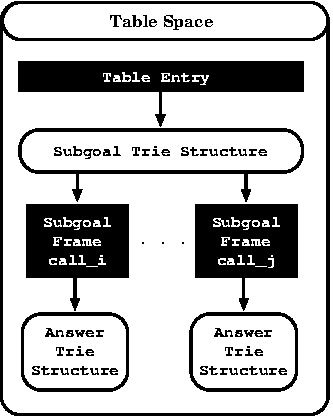
\includegraphics[width=4.5cm]{figures/table-space.pdf}
\caption{Table space organization}
\label{fig_table_space}
\vspace{-0.5\intextsep}
\end{wrapfigure}

Figure~\ref{fig_table_space} shows the table space organization of the
Yap system. At the entry point we have the \emph{table entry} data
structure. This structure is allocated when a tabled predicate is
being compiled, so that a pointer to the table entry can be included
in its compiled code. This guarantees that further calls to the
predicate will access the table space starting from the same
point. Below the table entry, we have the \emph{subgoal trie
  structure}. Each different tabled subgoal call to the predicate at
hand corresponds to a unique path through the subgoal trie structure,
always starting from the table entry, passing by several subgoal trie
data units, the \emph{subgoal trie nodes}, and reaching a leaf data
structure, the \emph{subgoal frame}. The subgoal frame stores
additional information about the subgoal and acts like an entry point
to the \emph{answer trie structure}. Each unique path through the
answer trie data units, the \emph{answer trie nodes}, corresponds to a
different answer to the entry subgoal.

%%%%%%%%%%%%%%%%%%%%%%%%%%%%%%%%%%%%%%%%%%%%%%%%%%%%%%%%%%%%%%%%%%%%%%
\subsection{Yap's Multithreaded Tabling Support}

Yap implements a SWI-Prolog compatible multi-threading
library~\cite{Wielemaker-03}. Like in SWI-Prolog, Yap's threads have
their own execution stacks and only share the code area where
predicates, records, flags and other global non-backtrackable data are
stored. 

In a multithreaded tabling evaluation, a thread views its tables as
private but, at the engine level, Yap has three designs that vary from
a \emph{No-Sharing} (NS) design, where each thread allocates fully
private tables for each new tabled subgoal called during its
computation, to a \emph{Full-Sharing} (FS), where threads share the
complete table space. Figure~\ref{fig_table_space} shows Yap's
multithreaded tabling support with an abstraction layer to which
threads interact (the threads represented in the bottom of the
figure), and at the engine level the configuration of the NS and FS
designs in a situation where several different threads evaluated the
same tabled subgoal call $i$. 

In the NS design, each thread allocates fully private tables for each
new subgoal called during its computation. One can observe that the
table entry data structure still stores the common information for the
predicate (such as the arity or the evaluation strategy), and then
each thread $t$ has its own cell $T_t$ inside a \emph{bucket array}
which points to the private data structures.

\begin{figure}[!ht]
\vspace{-\intextsep}
\centering
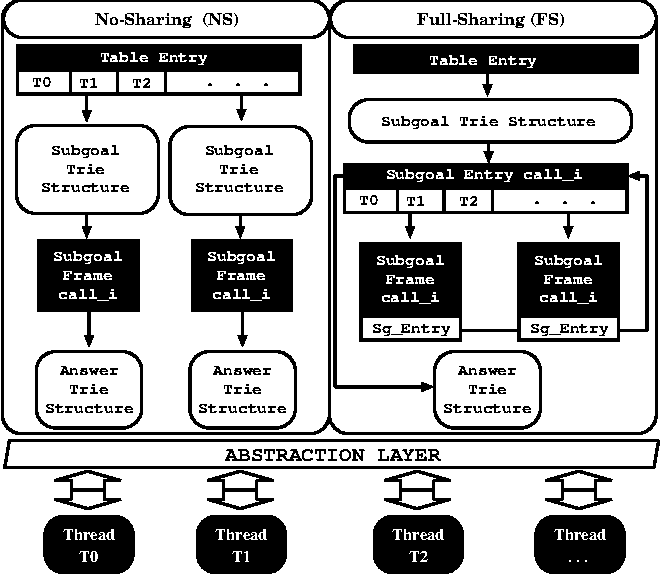
\includegraphics[width=9.5cm]{figures/yap-mt.pdf}
\caption{Yap's multithreaded tabled space using the NS and FS designs}
\label{fig_yap_mt_support}
\vspace{-1.0\intextsep}
\end{figure}

In the FS design, part of the subgoal frame information (the
\emph{subgoal entry} data structure) and the answer trie structure are
now shared among all threads. The previous subgoal frame data
structure was split into two: the \emph{subgoal entry} stores common
information for the subgoal call (such as the pointer to the shared
answer trie structure); the remaining information (the \emph{subgoal
  frame} data structure) remains private to each thread.

%%%%%%%%%%%%%%%%%%%%%%%%%%%%%%%%%%%%%%%%%%%%%%%%%%%%%%%%%%%%%%%%%%%%%%
\subsection{Scheduling Strategies}

The decision about the evaluation flow is determined by the
\emph{scheduling strategy}. Different strategies may have a
significant impact on performance, and may lead to a different
ordering of solutions to the query goal. Arguably, the two most
successful tabling scheduling strategies are \emph{local scheduling}
and \emph{batched scheduling}~\cite{Freire-96}.

Local scheduling strategy schedules the evaluation of a program in a
breath-first manner. It favors the backtracking first with completion
instead of the forward execution, leaving the consumption of answers
for last. Thus, it only allows a Cluster of Dependent Subgoals (CDS)
to return answers only after the completion point has been
reached~\cite{Freire-96}. %% In other words, the local scheduling tries
%% to keep a CDS as minimal as possible. When new answers are found, they
%% are added to the table space and the computation fails as consequence,
%% tabled subgoals inside a CDS propagate their answers to outside the
%% CDS only after its completion point is found.
Local scheduling causes a sooner completion of subgoals, which creates
less complex dependencies between them.

On the other hand, batched scheduling schedules the evaluation of a
program in a depth-first manner. It favors the forward execution first
instead of backtracking, leaving the consumption of answers and
completion for last. It thus tries to delay the need to move around
the search tree by batching the return of answers. When new answers
are found for a particular tabled subgoal, they are added to the table
space and the execution continues. For some situations, this results
in creating dependencies to older subgoals, therefore enlarging the
current CDS~\cite{Sagonas-98} and delaying the completion point to an
older generator node.

%%%%%%%%%%%%%%%%%%%%%%%%%%%%%%%%%%%%%%%%%%%%%%%%%%%%%%%%%%%%%%%%%%%%%%
\section{Extending Full-Sharing with Batched Scheduling}

In this section, we show how we have extended the FS design to support
batched scheduling. The usage of FS design with batched scheduling,
requires further support than with local scheduling, since when a new
answer is found it must be immediately propagated, and we have to
ensure that the propagation occurs on all subgoal calls once and only
once. To do so, next we show a procedure that, for every subgoal call
of every thread, keeps track of all the answers that were already
propagated.

%%%%%%%%%%%%%%%%%%%%%%%%%%%%%%%%%%%%%%%%%%%%%%%%%%%%%%%%%%%%%%%%%%%%%%
\subsection{Our Approach}

The key idea of our approach, which we named Privately-consumed Answer
Chaining (PAC), is then to extend the \emph{FS} design with batched
scheduling, by chaining privately for each subgoal call, the answers
that were already consumed by a thread. Since the procedure is
private, it will only affect the thread that is doing it. At the end,
when the evaluation is complete, i.e, when a subgoal call is marked as
complete, we put one of the private chain as public, so that from that
point on all threads can use that chain in complete (only reading)
mode.

Figure~\ref{fig_tabtries_pcc} shows the key data structures for
supporting the implementation of the PAC procedure during the
evaluation of a tabled subgoal call $i$ using the FS design. %% The FS
%% design, uses a subgoal entry data structure to store common
%% information for a subgoal call and a subgoal frame (\emph{SF}) data
%% structure to store private information about the execution of each
%% thread.
The PAC procedure works at the subgoal frame level, which is
private to each thread.

\begin{figure}[!ht]
\vspace{-\intextsep}
\centering
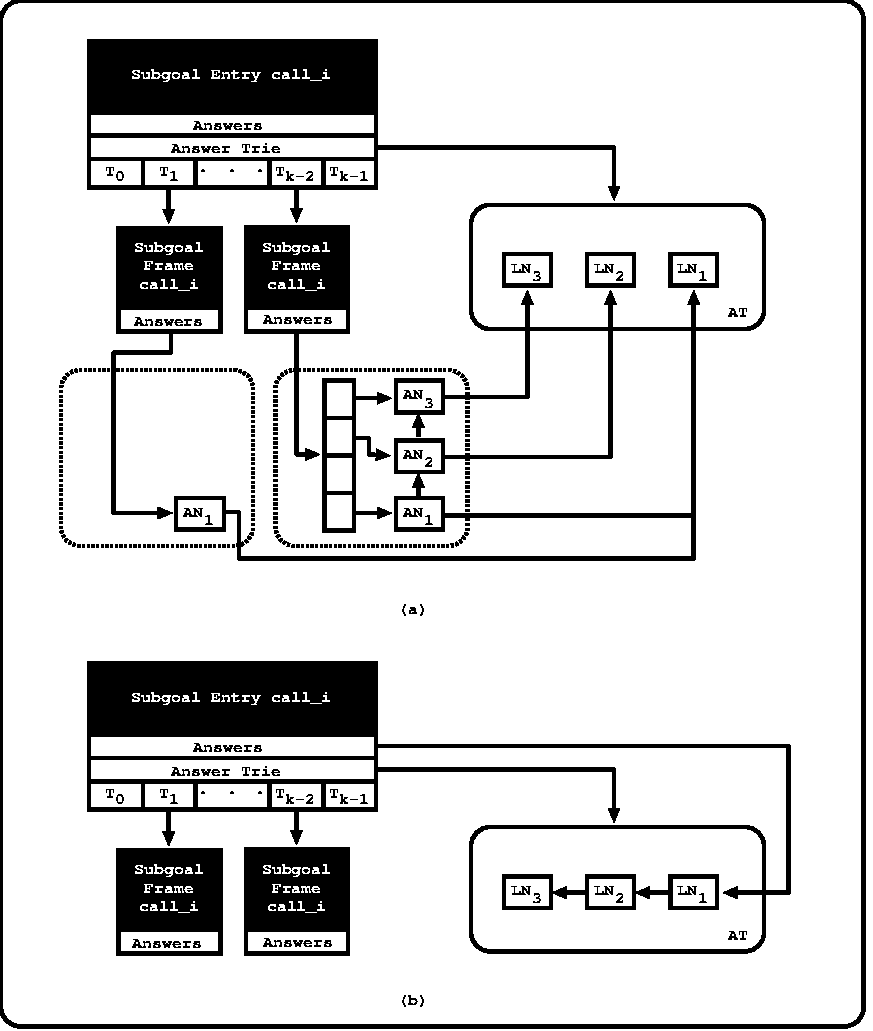
\includegraphics[width=10.5cm]{figures/pcc.pdf}
\caption{The \emph{FS} design with the PAC procedure - (a) private
  chaining and (b) public chaining}
\label{fig_tabtries_pcc}
\vspace{-1.0\intextsep}
\end{figure}

Figure~\ref{fig_tabtries_pcc}(a) shows then a situation where two
threads, $T_1$ and $T_{k-1}$, are sharing the same subgoal entry call
$i$ when the subgoal is still under evaluation, i.e., the subgoal is
not yet complete. The current state of the evaluation shows an answer
trie with $3$ answers found for the subgoal call $i$. For the sake of
simplicity, we are omitting the internal answer trie nodes and we are
only showing the leaf nodes nodes $LN_1$, $LN_2$ and $LN_3$, in the
figure. %% With the PAC procedure, the leaf nodes are not chained in the
%% answer trie data structure. Now, the chaining process is done
%% privately, and for that, we use the subgoal frame structure of each
%% thread.
On the subgoal frame structure we added a new field, called
\emph{consumer}, to store the answers found within the execution of
the thread. In order to minimize the impact of the \emph{PAC}
optimization, each node within the new consumer answer structure has
two fields: (i) an entry pointer, which points to the corresponding
leaf node in the answer trie data structure; (ii) a next pointer to
chain the answers within the consumer structure. To maintain a good
performance, when the number of nodes exceeds a certain threshold, we
use a hash trie mechanism design similar to the one presented in the
work~\cite{Areias-ijpp15}. However, since this mechanism is private to
each thread, it does not require any of the tools that were necessary
to support concurrency, thus we have removed them from the mechanism.

%% In particular, on each hash trie level, we
%% have removed the tools necessary to support concurrency, such as
%% useless pointers and compare-and-swap operations. We have chosen this
%% hashing mechanism, because it showed a good balance between lookup and
%% insert operations~\cite{Areias-ijpp15}, but the major reason was
%% mostly because of the integration in the TabMalloc memory
%% allocator~\cite{Areias-12b}.

Going back to Figure~\ref{fig_tabtries_pcc}(a), the consumer answer
structures represent then two different situations where threads can
be evaluating a subgoal call. Thread $T_1$ has only found one answer
and it is using a direct consumer answer chaining to access the node
$LN_1$. Thread $T_{k-1}$ was already found three answers for the
subgoal call and it is already using the hash trie mechanism within
its consumer answer structure. The consumer nodes are chained between
themselves, thus that consumer nodes belonging to thread $T_{k-1}$ can
consume the answers as in the original mechanism.

Figure~\ref{fig_tabtries_pcc}(b) shows the state of the subgoal call
after completion. When a thread $T$ completes a subgoal call, it frees
its private consumer structures, but before doing that, it checks
whether another thread as already marked the subgoal as completed. If
no other thread has done that, then thread $T$ not only follows its
private chaining mechanism as it would for freeing its private nodes,
but also, follows the pointers to the answer trie leaf nodes in order
to create a chain inside the answer trie. Since this procedure is done
inside a critical region, no more than one thread can be doing this
chaining process. Thus, in Figure~\ref{fig_tabtries_pcc}(b), we are
showing a situation where the subgoal call is completed and both
threads $T_1$ and $T_{k-1}$ have already removed their consumer answer
structures and chained the leaf nodes inside the answer trie.

%%%%%%%%%%%%%%%%%%%%%%%%%%%%%%%%%%%%%%%%%%%%%%%%%%%%%%%%%%%%%%%%%%%%%%
\subsection{Implementations Details}

At the tabling engine, the major difference between local and batched
scheduling is in the tabling operation \emph{tabled new answer}, where
we decide what to do when an answer is found during the
evaluation. This operation checks whether a newly found answer is
already in the corresponding answer trie structure and, if not,
inserts it. Algorithm~\ref{alg_table_new_answer_batched} shows how we
have extended this operation to support FS design with batched
scheduling.

\begin{algorithm} [!ht]
\caption{tabled\_new\_answer(answer ANS, subgoal frame SF)}
\algsetup{indent=0.65cm}
\begin{algorithmic}[1]
  \STATE $leaf \gets check\_insert\_answer\_trie(ANS, SF)$
  \STATE $chain \gets check\_insert\_consumer\_chain(leaf, SF)$
  \IF {$is\_answer\_marked\_as\_found(chain) = True$}
    \RETURN $failure$
  \ELSE                                        [the answer is new]
    \STATE $mark\_answer\_as\_found(chain)$
    \IF {$local\_scheduling\_mode(SF)$}
      \RETURN $failure$
    \ELSE                                [batched scheduling mode]
      \RETURN $proceed$
    \ENDIF
  \ENDIF  
\end{algorithmic}
\label{alg_table_new_answer_batched}
\end{algorithm}

The algorithm receives two arguments: the new answer found during the
evaluation (\emph{ANS}) and the subgoal frame which corresponds to the
call at hand (\emph{SF}). The algorithm begins by checking/inserting
the given \emph{ANS} into the answer trie structure, which will return
the leaf node for the path representing \emph{ANS} (line 1).

Then, it checks/inserts the given \emph{leaf} node into the private
consumer chain for the current thread, which will return the
corresponding chain node (line 2). Next in line 3, it tests whether
the chain node already existed in the consumer chain, i.e., if it was
inserted or not by the current check/insert operation in order to
return failure (line 4), or it proceeds with marking the answer
\emph{ANS} has found (line 6). At the end (lines 7 to 10), it returns
failure if local scheduling is active (line 8), otherwise, the batched
scheduling is active, thus it propagates the answer \emph{ANS} (line
10).

%%%%%%%%%%%%%%%%%%%%%%%%%%%%%%%%%%%%%%%%%%%%%%%%%%%%%%%%%%%%%%%%%%%%%%
\section{Performance Analysis}

We now present experimental results about the usage of the batched
scheduling on FS design. To put results in perspective, we will be
showing also the results for the NS design. The environment for our
experiments was a machine with 32-Core AMD Opteron (TM) Processor 6274
(2 sockets with 16 cores each) with 32G of main memory, running the
Linux kernel is the 3.16.7-200.fc20.x86\_64 with Yap 6.3.

For the experimentation, we used our memory allocator described in the
work~\cite{Areias-12b}, later named \emph{TabMalloc}, and we the same
five sets of benchmarks. These benchmarks create \emph{worst case}
scenarios, where we are able to show the lowest bounds in terms of
performance that each design might achieve when applied/used with
other real world applications/programs.

Table~\ref{tab_batched_overhead} shows the overhead ratios, when
compared with the NS design with 1 thread (running with local
scheduling without TabMalloc), for the NS and FS designs, when running
1, 8, 16, 24 and 32 threads, with TabMalloc and, local scheduling
(column \emph{Local}) and batched scheduling (column \emph{Batched})
strategies. In order to give a fair weight to each benchmark, the
overhead ratio is calculated as follows. We begin by running ten times
each benchmark $B$ for each design $D$ with $T$ threads. Then, we
calculate the average of those ten runs and use that value ($D_{BT}$)
to put it in perspective against the base time, which is the average
of the ten runs of the NS design with $1$ thread ($NS_{B1}$). For
that, we use the following formula for the overhead $O_{DBT} = D_{BT}
/ NS_{B1}$.  After calculating all the overheads $O_{DBT}$ for a
certain design $D$ and number of threads $T$ corresponding to the
several benchmarks $B$, we calculate the respective minimum, average,
maximum and standard deviation overhead ratios.

\setlength{\tabcolsep}{12pt}
\begin{table}[!ht]
\vspace{-\intextsep}
\centering
%% \caption{Overhead ratios, when compared with the NS design with $1$
%%   thread (running with local scheduling without TabMalloc) for the NS
%%   and FS designs (with TabMalloc), when running 1, 8, 16, 24 and 32
%%   threads with local and batched scheduling on the five sets of
%%   benchmarks (best ratios by row and by design for the Minimum,
%%   Average and Maximum are in bold)}
\caption{Overhead ratios, when compared with the NS design with 1
  thread for the NS and FS designs, when running 1, 8, 16, 24 and 32
  threads with local and batched scheduling (lowest is the best and it
  is marked in bold by row and by design for the Minimum, Average and
  Maximum)}
\vspace{-0.5\intextsep}
%\scalebox{1.00} {
\begin{tabular}{ll|cc|cc}
\hline\hline
\multicolumn{2}{c|}{\multirow{2}{*}{\bf Threads}} &
\multicolumn{2}{c|}{\multirow{1}{*}{\bf NS}} &
\multicolumn{2}{|c}{\multirow{1}{*}{\bf FS}}\\ \cline{3-6}
& 
& \multicolumn{1}{c}{\bf Local}
& \multicolumn{1}{c}{\bf Batched}
& \multicolumn{1}{|c}{\bf Local}
& \multicolumn{1}{c}{\bf Batched}\\
\hline
\multirow{4}{*}{\bf 1}
& {\bf Min }& {\bf 0.53}& 0.55& 1.01& {\bf 0.95}\\
& {\bf Avg }& {\bf 0.78}& 0.82& {\bf 1.30}& 1.46\\
& {\bf Max }& 1.06& {\bf 1.05}& {\bf 1.76}& 2.33\\
& {\bf StD }& 0.15& 0.14& 0.22& 0.44\\
\hline
\multirow{4}{*}{\bf 8}
& {\bf Min }& 0.66& {\bf 0.63}& 1.16&{\bf  0.99}\\
& {\bf Avg }& {\bf 0.85}& 0.88& {\bf 1.88}& 1.95\\
& {\bf Max }& {\bf 1.12}& 1.14& {\bf 2.82}& 3.49\\
& {\bf StD }& 0.13& 0.14& 0.60& 0.79\\
\hline
\multirow{4}{*}{\bf 16}
& {\bf Min }& 0.85& {\bf 0.75}& 1.17& {\bf 1.06}\\
& {\bf Avg }& {\bf 0.98}& 1.00& {\bf 1.97}& 2.08\\
& {\bf Max }& {\bf 1.16}& 1.31& {\bf 3.14}& 3.69\\
& {\bf StD }& 0.09& 0.17& 0.65& 0.83\\
\hline
\multirow{4}{*}{\bf 24}
& {\bf Min }& {\bf 0.91}& 0.93& 1.16& {\bf 1.09}\\
& {\bf Avg }& {\bf 1.15}& 1.16& {\bf 2.06}& 2.19\\
& {\bf Max }& 1.72& {\bf 1.60}& {\bf 3.49}& 4.08\\
& {\bf StD }& 0.20& 0.21& 0.70& 0.91\\
\hline
\multirow{4}{*}{\bf 32}
& {\bf Min }& 1.05& {\bf 1.04}& 1.33& {\bf 1.26}\\
& {\bf Avg }& 1.51& {\bf 1.49}& {\bf 2.24}& 2.41\\
& {\bf Max }& {\bf 2.52}& 2.63& {\bf 3.71}& 4.51\\
& {\bf StD }& 0.45& 0.45& 0.74& 1.02\\
\hline\hline
\end{tabular}%}
\label{tab_batched_overhead}
\vspace{-0.7\intextsep}
\end{table}

By observing Table~\ref{tab_batched_overhead}, we can see that, for 1
thread, on the minimum overhead ratio, local scheduling is better on
the NS design, while batched scheduling is better in the FS
design. For the average and maximum overhead ratios, in the FS design,
the best strategy is always the local scheduling.   

As we scale the number of threads, for the NS design both scheduling
strategies have similar minimum, average and maximum overhead
ratios. For the FS design, the best minimum overhead ratio is always
for the batched scheduling. For the average and maximum overhead
ratio, local scheduling is always better than batched
scheduling. However, for the average ratio, the results between both
strategies is quite close. For the maximum overhead ratio, the
difference between both strategies is significantly higher. 

%%  As we scale the number of threads, one can observe that,
%% for the NS design both scheduling strategies have similar minimum,
%% average and maximum overhead ratios. For the FS design, the best
%% minimum overhead ratio on $1$, $8$, $16$, $24$ and $32$ threads is
%% always the batched scheduling. For the average and maximum overhead
%% ratio, local scheduling is always better than batched
%% scheduling. However, for the average ratio, the results between both
%% strategies is quite close. We consider this to be quite significant,
%% once the FS design with batched scheduling requires the support of the
%% PAC procedure. For the maximum overhead ratio, the difference between
%% both strategies is higher than for the average overhead ratio, however
%% we hope to reduce the difference with further improvements in the PAC
%% procedure.

%%%%%%%%%%%%%%%%%%%%%%%%%%%%%%%%%%%%%%%%%%%%%%%%%%%%%%%%%%%%%%%%%%%%%%
\section{Conclusions and Further Work}
We have presented a simple and novel approach for combining the FS
design with batched scheduling. Experimental results showed that on
average, the extra structures required for the combination do not seem
to have a big impact in the performance. Further work will include
experimentation in other real world applications.

%%%%%%%%%%%%%%%%%%%%%%%%%%%%%%%%%%%%%%%%%%%%%%%%%%%%%%%%%%%%%%%%%%%%%%

%\section*{Acknowledgments}

%%%%%%%%%%%%%%%%%%%%%%%%%%%%%%%%%%%%%%%%%%%%%%%%%%%%%%%%%%%%%%%%%%%%%%

\bibliographystyle{splncs}
\bibliography{references}

%%%%%%%%%%%%%%%%%%%%%%%%%%%%%%%%%%%%%%%%%%%%%%%%%%%%%%%%%%%%%%%%%%%%%%

\end{document}
